\documentclass{article}
\usepackage[utf8]{inputenc}
\usepackage[a4paper, margin=2.5cm]{geometry}
\usepackage{graphicx}
\usepackage[french]{babel}

\usepackage[default,scale=0.95]{opensans}
\usepackage[T1]{fontenc}
\usepackage{amssymb} %math
\usepackage{amsmath}
\usepackage{amsthm}
\usepackage{systeme} %use with \system*{eq1, eq2}
\usepackage{bbm}

\usepackage{import}
\usepackage{xifthen}
\usepackage{pdfpages}
\usepackage{transparent}



\newcommand{\incfig}[2][1]{%
    \def\svgwidth{#1\columnwidth}
    \import{./figures/}{#2.pdf_tex}
}

\usepackage{hyperref}
\hypersetup{
    colorlinks=true,
    linkcolor=blue,
    filecolor=magenta,      
    urlcolor=cyan,
    pdftitle={Overleaf Example},
    %pdfpagemode=FullScreen,
}
\urlstyle{same} %\href{url}{Text}

\theoremstyle{plain}% default
\newtheorem{thm}{Théorème}[section]
\newtheorem{lem}[thm]{Lemme}
\newtheorem{prop}[thm]{Proposition}
\newtheorem*{cor}{Corollaire}
%\newtheorem*{KL}{Klein’s Lemma}

\theoremstyle{definition}
\newtheorem{defn}{Définition}[section]
\newtheorem{exmp}{Exemple}[section]
%\newtheorem{xca}[exmp]{Exercise}

\theoremstyle{remark}
\newtheorem*{rem}{Remarque}
\newtheorem*{note}{Note}
%\newtheorem{case}{Case}



\title{Cours}
\author{Charles Vin}
\date{Date}

\begin{document}
\maketitle

\section{Rappel avec le poly}

\subsection{Mesure}
Exemple 1.4 :
\begin{itemize}
    \item Lebesgue :  $ \phi ([a,b]) = b-a $ 
    \item Dirac :  $ \delta_x = \delta_x(A) = 1_A(x)$ 
    \item Mesure de comptage : C(A) = \systeme*{+\infty \text{ si A infiny}, card(A) \text{sinon}} 
\end{itemize}

4) Mesure discrète : Somme de masse de Dirac 
$ \mu = \sum_{i \in I}^{p_i\delta_i} $ (99\% du temps  $ I=N $ )

5) Mesure à densité :
Soit f une fonction > 0 \\ 
\[
    \mu _f = fdx \Leftrightarrow \mu _f(A) = \int_{A} f(x)dx
.\]

Que signifie  $ \int fd \mu  $ ? \\
Si  $ \mu  = dx  $ alors  $ \int_{}^{} fdx = \int_{}^{}f(x)dx$\\
Si  $ \mu  = \delta _x $ alors  $ \int_{}^{}f d \delta _x = f(x)$ car  $ \delta_x  $ "met que du poids en x" \\
Si  $ \mu = \mu _a + \mu _2 $ alors  $ \int_{}^{}f d \mu = \int_{}^{} f d \mu _1 + \int_{}^{} f d \mu _2 $ \\
Si  $ \mu = (1-p) \delta _0 + p \delta _1 $ alors  
\begin{align*}
    \int_{}^{} f d \mu &= \int_{}^{}f (1-p )\delta _0 + \int_{}^{} f p \delta _1 \\
                        &= (1-p)\int_{}^{}f \delta _0 + p \int_{}^{} f \delta _1 \\
                        &= (1-p)f(0) + pf(1)
\end{align*}

Rappels de L2 \\
Si  $ \mu $  à une densité g alors :
\begin{gather*}
    \mu  = gdx \text{ avec } g(x)= (1-x) \mathbbm{1}_{[0,1]}(x) \\
    \int_{}^{}fd \mu  = \int_{}^{} f(x)g(x)dx
\end{gather*}
exemple :  $ f(x) = (1-x)^3 $ \\
on a alors \begin{align*}
    \int_{}^{}fd \mu  &= \int_{}^{} (1-x)^3 \mathbbm{1}_{[0,1]}(x) * (1-x) \\
                    &= \int_{0}^{1}(1-x)^4 dx = 1/5
\end{align*}

Dernier exemple : \\
Si  $ \mu  = \frac{1}{2} \mathbbm{1}_{[0,1]}(x)dx + \frac{1}{2} \delta _3  $ alors \begin{align*}
    \int_{}^{}fd \mu &= \frac{1}{2} \int_{}^{}f \mathbbm{1}_{[0,1]}(x) dx  + \frac{1}{2} \int_{}^{}f \delta _3 \\
                    &= \frac{1}{2} \int_{0}^{1} f(x)dx + \frac{1}{2} f(3)
\end{align*} 

\subsection{Variable aléatoire}
Exemple : \begin{itemize}
    \item Si  $ X \sim Bern(p), P_x = (1-p) \delta _0 + p \delta _1$ on a  $ P_x([2,+ \infty[) = P(X \in [2, + \infty ]) = 0 $  
    \item Si  $ X \sim  N(0,1) $ alors  $ P_X = \frac{1}{\sqrt[]{\pi }}e^{-\frac{x^2}{2}} dx $ 
    \item En général, la loi d'une variable aléatoire discrète à valeur dans N : 
    \[
        P_X = \sum_{}^{} P(X=1) \delta _1 ????????
    .\]
    Soit  $ B(p) $ 
\end{itemize}


\begin{defn}[Moment d'une VAR]
    Si X discrète : 
    \[
        E(X) = \sum_{k=0}^{\infty }kP(X=k)
    .\]
    Si X à densité $ fdx $ 
    \[
        E(X) = \int_{R}^{}xf(x)dx = \int_{}^{}xdP_x \text{ = Nouvelle notation}
    .\]
    
    Preuve que la nouvelle notation unifie les deux formules de l'esperance : \begin{proof}[Preuve : ]
        \begin{itemize}
            \item Pour la densité : $ X $ de densité $ f_X $ et $ P_x = f_X dx $ 
            \[
                \int_{}^{}gdP_X = \int_{}^{}gf_X dx = \int_{}^{}g-x)f(x) dx 
            .\]
            Si $ g(x) = x $ alors 
            \[
                \int_{}^{}xdP_X = \int_{}^{}xf_X(x)dx = E(X)
            .\]
            
            \item Pour une VA discrète : échaufement avec Bernouilli : $ P_x = (1-p)\delta _0 + p \delta _1$ 
            \[
                E(X) = \sum_{k=0}^{\infty } kP(X=k)=0+P+0 = p
            .\] 
            \begin{align*}
                \int_{}^{}xdP_x = (1-p)\int_{}^{}xd? + p \int_{}^{}x \delta _1 = p \\
                                &= (1-p)*0 + p = p 
            \end{align*}
            Fin de l'échauffement : 
            \[
                \int_{}^{}xdP_X \text{ si } P_X = \sum_{k=0}^{\infty }P(X=k) \delta _k
            .\]
            
            
            \begin{align*}
                \int_{}^{}xdP_X &= \sum_{k=0}^{\infty }\int_{}^{}xP(X=k) \delta _k \\
                &= \sum_{}^{}P(X=k) \int_{}^{}x \delta _k
                &= \sum_{}^{}P(X=k) * k = E(X)            
            \end{align*}      
            
        \end{itemize}
    \end{proof}

    \textbf{Formule général}
    \begin{align*}
        E(g(X)) = \int_{}^{}gdP_X \\
        E(X^2) = \int_{}^{}x^2 dP_X = \systeme*{
            \int_{}^{}x^2 f(x) dx ,
            \sum_{}^{}k^2 P(X)k
        }        
    \end{align*}
    \begin{note}[]
        Le systeme représente soit l'un soit l'autre en fonction de densité ou discrète
    \end{note}
\end{defn}

\begin{exmp}[]
    $ P_X = \frac{1}{2}\delta _1 + \frac{1}{2} \frac{1}{\sqrt[]{\pi }} e^{-\frac{x^2}{2}} dx $ \begin{align*}
        E(g(x)) &= \int_{}^{}gdP_X \\
                &= \frac{1}{2} \int_{}^{}g \delta _1 + \frac{1}{2} \int_{}^{}g(x) \frac{1}{\sqrt[]{\pi }} e^{-\frac{x^2}{2}} dx \\
                &= \frac{1}{2} g(1) + \frac{1}{2} \int_{}^{}g(x) \frac{1}{\sqrt[]{\pi }} e^{-\frac{x^2}{2}} dx \\
    \end{align*}
\end{exmp}

\subsection{Indépendance}
$ X \perp Y \Leftrightarrow E(f(X)g(Y)) = E(f(X)) E(g(X))$


\section{Loi des grand nombres et intervalles de confiance }
BUT : \begin{itemize}
    \item $ X, ..., X _{n} $ VA iid 
    \[
        \bar{X_n} = \frac{1}{n} \sum_{i=1}^{n}X_i 
    .\]
    Que dire de la suite $ (\bar{X_n}) $ ? 

    \item Si on cherche à estimer une quantité inconnu $ \theta  $. On cherche $ I $ tel que : 
    \[
        P(\theta \in I) \geq 0.95
    .\]
    
    \begin{exmp}[]
        On a une pièce et on veut savoir si elle est équilibrée. \\ 
        On modelise le résultat de cette pièce par une variable aléatoire de Bernouilli de paramètre $ p $ (p est inconnu) \\
        0 $\rightarrow$ pile \\
        1 $\rightarrow$ face \\

    \end{exmp}
    IL MANQUE DES TRUCS SQDGQRZG3A
\end{itemize}


\subsection{Inégalité de concentration}
\begin{thm}[Inégalité de Markov]
    Soit $ X $ une variable aléatoire définie sur un espace probabilisé $ (\Omega , F, \pi ) $. \begin{itemize}
        \item $ X $ est positive (X est à valeur dans $ R^+ $ ) (espace de dépard dans R+)
        \item X admet une espérance ($ 0 \leq E(X) \leq + \infty  $ )
    \end{itemize}
    Alors on a : 
    \[
        \forall t > 0, P(X \geq t) \leq \frac{E(X)}{t}
    .\]
    
    \begin{proof}[Preuve : ]
        Soit $ X $ une va positive, d'espèrance finie. Soit $ t > 0 $ :
        \[
            P(X > t) = E(\mathbbm{1}_{[t, +\infty[}(X)))
        .\]
        On sais que : 
        \[
            \forall x \geq 0, \forall t > 0, \mathbbm{1}_{[t, +\infty[} \leq \frac{x}{t} \mathbbm{1}_{[t, +\infty[} \leq \frac{x}{t}
        .\]
        On peut dessiner les courbes pour comprendre l'inéquation.\\
        On a donc : 
        \[
            \forall t > 0, \mathbbm{1}_{[t, +\infty[} \leq \frac{X}{t}
        .\]
        Par croissance de l'espérance, on a : 
        \[
            \forall t > 0, E(\mathbbm{1}_{[t, +\infty[}) = P(X \geq t) \leq \frac{E(X)}{t}
        .\]
    \end{proof}
\end{thm}

\begin{thm}[Inégalité de Tchebychev]
    \begin{note}[Moment d'odre p]
        X admet un moment d'ordre 2
        \[
            \Leftrightarrow E(\left| X \right| ^2) < + \infty 
        .\]
        Moment d'ordre p : 
        \[
            \Leftrightarrow E(\left| X \right| ^p ) < + \infty 
        .\]
    \end{note}
    Soit $ X $ une var définie sur un espace $ (Omega, F, P) $ qui admet un moment d'ordre deux. On a :  
    \[
        \forall t > 0, P(\left| X-E(X) \right| \geq t) \leq \frac{Var(X)}{t^2}
    .\]
    \begin{proof}[Preuve: ]
        Soit $ X $ une var admettant un moment d'ordre 2.\\
        Soit $ Y=(X-E(X))^2 $\begin{itemize}
            \item Y est une variable positive
            \item $ E(Y) = Var X < + \infty $ 
        \end{itemize}
        D'après l'inégalité de Markov 
        \[
            P(Y \geq y) \leq \frac{E(Y)}{y} = \frac{Var X}{u}
        .\]
        Soit $ t>0 $  
        \[
            P(\left| X-E(X) \right| \geq t ) \Leftrightarrow P((X-E(X))^2 \geq t^2)
        .\]
        D'après l'inégalité précédente avec $ u = t^2 > 0 $ on a : 
        \[
            P(\left| X-E(X) \right| \geq t) \leq \frac{Var X}{t^2}
        .\]        
    \end{proof}
\end{thm}

\begin{exmp}[]
    Si $ X ~ \mathcal{N}(3,5) $ : 
    \[
        P(\left| X-3 \right| \geq 7) \leq \frac{Var X}{7^2} = \frac{5}{49}
    .\]    
\end{exmp}
\begin{exmp}[]
    Si $ X ~ \mathcal{E}(\lambda )  $ : 
    \[
        \forall t>0, P(\left| X-\frac{1}{\lambda } \right| \geq t) \leq \frac{1}{\lambda ^2 t^2}
    .\]
\end{exmp}
\begin{exmp}[\textbf{MEILLEURS EXEMPLE GIGA IMPORTANT}]
    $ X_1, ... ,X_n $ va iid de loi $ \mathcal{B}(p) p$ inconnu 
    \[
        \bar{X_n} = \frac{1}{n}\sum_{i=1}^{n}X_i
    .\]
    \begin{align*}
        E(\bar{X_n}) &= E(\frac{1}{n}\sum_{i=1}^{n}X_i) \\
                    &= \frac{1}{n} E(\sum_{i=1}^{n}X_i) \\
                    &= \frac{1}{n}\sum_{i=1}^{n}p = p
    \end{align*}
    Que vaut la variance de $ \bar{X_n} $ ?
    \begin{align*}
        Var \bar{X_n} &= Var (\frac{1}{n} \sum_{i=1}^{n}X_i) \\
                    &= \frac{1}{n^2} Var(\sum_{i=1}^{n}X_i) \\
                    &= \frac{1}{n^2}\sum_{i=1}^{n}Var(X_i) \\
                    &= \frac{1}{n^2}n*(p*(1-p))
    \end{align*}
    
    \[
        Var(\bar{X_n}) = \frac{p(1-p)}{n}
    .\]
    On applique l'inégalité de Tchebychev : 
    \begin{align*}
        \forall t>0, P(\left| \bar{X_n}-p \right|  \geq t) & \leq \frac{p(1-p)}{nt^2} \\
                & \leq \frac{1}{4nt^2}
    \end{align*}
    On reviendra sur cette exemple dans deux définition
\end{exmp}
    
\begin{defn}[Intervalle de confiance ]
    Pour un modèle statistique $ \Omega, F, (P_{\theta })_{\theta \in \Theta } $ et une quantité à estimer $ g(\theta ) $, un intervalle de confiance de niveau $ 1-\alpha, \alpha \in [0,1] $ est un intervalle $ I(X_1, ..., X_n) $ construit à partir de $ X_i $ tel que 
    \[
        \forall \theta  \in \Theta , P(\theta \in I(X_1, \dots, X _{n} )) \geq 1- \alpha 
        .\]
        où $ X_1, \dot, X _{n}  $ sont des variables iid qui servent à construire l'estimateur
    \end{defn}
    \begin{exmp}[Retour sur l'exemple]
        Construison ensemble un intervale de confiance pour $ p $ de niveau 0.99 ($ \alpha = 0.01 $ d'erreur acceptée).\\
        On sait que 
        \[
            \forall t > 0, P(\left| \bar{X_n}-p \right| > t) \leq \frac{1}{4nt^2}
            .\]
            cela signifie qu'avec proba au moins $ 1-\frac{1}{4nt^2} $ on a 
            \begin{align*}
                \left| \bar{X_n}-p \right| < t \\
                &\Leftrightarrow p \in ]\bar{X_n} - t, \bar{X_n} + t [ \\
                &\Leftrightarrow P(p \in ]\bar{X_n} - t, \bar{X_n} + t [ ) \geq 1-\frac{1}{4nt^2}
            \end{align*}
            Or on cherche avec un niveau $ \alpha = 0.01 $ 
    \[
        \alpha = \frac{1}{2 \sqrt[]{\alpha n}}
    .\]
    
    \[
        \forall p \in [0,1], P(p \in ] \bar{X_n}- \frac{1}{2 \sqrt[2]{\alpha n}}; \bar{X_n}+ \frac{1}{2 \sqrt[]{\alpha n}}[)
    .\]
    Avec $ \alpha = 0.01$ cela devient : 
    \[
        p \in ] \bar{X_n}- \frac{1}{0.2 \sqrt[2]{n}}; \bar{X_n}+ \frac{1}{0.2 \sqrt[]{n}}[
    .\]
\end{exmp}
\begin{exmp}[]
    je veux une précision de $ 0.04 $ sur $ p $. Comment choisir $ n $ ? $ n $ est solution de 
    \begin{align*}
        0.04 = \frac{1}{2 \sqrt[]{\alpha n}} = \frac{1}{2*0.2 * \sqrt[]{n}} \\
        0.4*0.04 = \frac{1}{\sqrt[]{n}} \\
        \Leftrightarrow n= \frac{1}{(0.4*0.04)^2} \approx 4000
    \end{align*}
\end{exmp}

\begin{defn}[Convergence en probabilité]
    Soit $ (X_m)_{n \in N} $ une suite de va définie sur $ (\Omega, F, P) $ . Soit $ X $ une va définie sur $ (\Omega, F, P) $.  \\
    On dit que $  (X_m)_{n \in N} $ converge en probabilité vers $ X $ si 
    \[
        \forall t > 0, P(\left| X_n - X \right| \geq t) \rightarrow_{n \rightarrow \infty } 0
    .\]
    On le note $ X_n \rightarrow_{n \rightarrow + \infty }^P X$ 
\end{defn}   

\begin{thm}[Loi faible des grands nombre]
    Soit $ (X_n)_{n \in N} $ une suite de va définie sur $ (\Omega, F, P) $. \\
    Si $ X $ admet un moment d'ordre 2. Alors 
    \[
        \frac{1}{n} \sum_{x=1}^{n} X_i \rightarrow_{n \rightarrow + \infty }^P E(X_i)
    .\]
    C'est à dire :
    \[
        \forall t > 0, P(\left| \frac{1}{n}\sum_{i=1}^{n}X_i -E(X) \right| \geq t) \rightarrow_{n \rightarrow + \infty } 0
    .\]
\end{thm}

\begin{proof}[Preuve: ]
    Soit $ (X_i)_{i \in N} $ une suite de v.a.r iid, admettant une espérance $ m $ et une variance. \\
    Soit $ \bar{X_n} = \frac{1}{n}\sum_{i=1}^{n}X_i $ 
    \begin{enumerate}
        \item Calculons $ E(\bar{X_n}) $ \begin{align*}
            E(\bar{X_n}) &= E(\frac{1}{n}\sum_{i=1}^{n}X_i) \\
                    &= \frac{1}{n}\sum_{i=1}^{n}E(X_i) \\
                    &= \frac{n}{n}*m = m 
        \end{align*} 
        \item Calculons $ Var(\bar{X_n}) $ \begin{align*}
            Var(\bar{X_n}) &= Var(\frac{1}{n}\sum_{i=1}^{n}X_i) \\
                        &= \frac{1}{n^2}Var(\sum_{i=1}^{n}X_i) \\
                        &= \frac{1}{n^2} \sum_{i=1}^{n} Var(X_i)\\
                        &= \frac{n}{n^2}Var(X_i) = \frac{Var(X_1)}{n}
        \end{align*} 
    \end{enumerate}
    D'après l'inégalité de Tchebytchev appliqué à $ \bar{X_n} $ (qui possède une variance finie), on a : 
    \[
        \forall t>0, P(\left| \bar{X_n}-E(X) \right| \geq t) \leq \frac{Var(X_1)}{nt^2} \longrightarrow _{n \to +\infty } 0
    .\]
\end{proof}

\begin{exmp}[]
    Si $ (X_i)_{i \in N} $ est une suite iid de variable de la $ \mathcal{B}(p) $. Que dire de $ \frac{1}{n}\sum_{i=1}^{n}X_i $ ? $E(X_1) = p , Var(X_1)= p(1-p) < \infty$
    D'après la loi faible des grands nombres : 
    \[
        \frac{1}{n} \sum_{i=1}^{n}X_i \to_{n \to \infty }^\mathcal{P} p 
    .\]
\end{exmp}
\begin{exmp}[]
    Si les $ X_i $ sont des va iid de la loi $ \mathcal{N}(0,1) $, $ E(X_1) = 0, Var(X_1) = 1 $ 
    \[
        \frac{1}{n}\sum_{i=1}^{n}X_i \to_{n \to \infty }^\mathcal{P} 0
    .\]
    Si les $ X_i $ sont iid de la loi $ \mathcal{E}(\lambda ),\lambda >0 $ Ainsi 
    \[
        \frac{1}{n}\sum_{i=1}^{n}X_i \to_{n \to \infty }^\mathcal{P} \frac{1}{\lambda }
    .\]
    Si les $ X_i $ de loi $ \mathcal{B} (m,p) $ 
    \[
        \frac{1}{n}\sum_{i=1}^{n}X_i \to_{n \to \infty }^\mathcal{P} mp
    .\]
\end{exmp}
Quelque exemple de convergence en probabilités \begin{itemize}
    \item $ (X_n) $ à $ X_n $ a une loi $\mathcal{B}(\frac{1}{n})$ Vers quoi $ X_n $ converge ? \\ 
    Soit $ t>0 $ fixé, $ P(\left| X_n-0 \right| \geq t) = P(X_n=1) = \frac{1}{n} \to _{n \to \infty } 0 $ (Aussi faisable ave Tchebychev) 
    \item Si $ X_n $ soit une v.a de la loi $ \mathcal{E}(n) $ 
    \[
        f_{X_n}(n) = ne^{-nx} \mathbb{1}_{x \geq 0}()
    .\]
    On se doute que $ X_n \to_{n \to \infty }^\mathcal{P} 0 $ 
    \[
        \forall t > 0, P(\left| X_n \right| \geq t) = \int_{t}^{+\infty }ne^{-xn} dx = \int_{tn}^{+\infty } e^{-u} du = e^{-tn} \to_{n \to \infty } 0
    .\]    
\end{itemize}

\begin{rem}[]
    La convergence en probabilité est la notion de convergence la plus faible du cours. \\ 
    Si $ X_n \to_{n \to \infty }^\mathcal{P} X $, je ne sais pas, elle n'implique pas $ E(X_n) \to_{n \to \infty } E(X) $  
\end{rem}

\section{Loi forte des grands nombres}
\begin{defn}[Ensemble négligeable et ensembles presque-sûrs]
    Soit $ (\Omega, F, P) $ un espace probabilisé. \\
    On dit que $ A \in F $ est \textbf{négligeable} si $ P(A) = 0 $ \\
    On dit que $ B \in F $ est \textbf{presque-sûr} si $ P(B) = 1 $ 
\end{defn}
\begin{exmp}[]
    $ \Omega = \{0,1\}^{\mathbb{N}}  F=P(\omega ), A=\{w \in \Omega ,\forall i \in N, w_i = 1\}$ , $ P(A) = 0 $ ? (proba d'une infinité de pile ou face avec proba 1/2)
    \[
        P(A_N) = \frac{1}{2^N}, P(A) = P(\bigcap_{N \in N}^{}) = \lim_{n \to \infty} P(A_n) = 0 
    .\]
\end{exmp}
\begin{exmp}[]
    $ X $ v.a uniforme sur [0,1]
    \[
        A=\{\frac{1}{2}\}, P(A) = P(X=\frac{1}{2}) = 0
    .\]
    
    \[
        P(X \in ]\frac{1}{2}-\epsilon , \frac{1}{2} + \epsilon [) = 2 \epsilon = \int_{1/2-\epsilon }^{1/2+\epsilon } 1dx
    .\]    
\end{exmp}
\begin{rem}[]
    Un ensemble négligeable n'est a priori pas vide.
\end{rem}
\begin{thm}[]
    Soit $ (A_n) $ une suite d'ensemble négligeable.
    \begin{itemize}
        \item $\bigcup_{n \in N}^{}A_n$ est un ensemble négligeable
        \item $\bigcap_{n \in N}^{}A_n$ est un ensemble négligeable.
    \end{itemize}
    \begin{proof}[Preuve: ]
        \begin{itemize}
            \item $ 0 \leq P(\bigcup_{n \in N}^{}) \leq \sum_{n \in N}^{} P(A_n) = 0 $ 
            \item $ 0 \leq P(\bigcap_{n \in N}^{}) \leq \sum_{n \in N}^{} P(A_n) = 0 $ car $ \bigcap_{n \in N}^{}A_n \subset A_1 $ 
        \end{itemize}
    \end{proof}
    \begin{cor}[immédiat]
        Si les $ (B_n)_{n \in N} $ sont presque sur : \begin{itemize}
            \item $ \bigcap_{n \in N}^{} B_n $ est presque-sûrs
            \item $ \bigcup_{n \in N}^{} B_n $ est presque-sûrs 
        \end{itemize}
    \end{cor}
    
    \begin{defn}[Convergence presque-sûr]
        Soit $ (X_n)_{n \in N} $ une suite de variables aléatoire définis sur $ (\Omega , F, P) $ \\
        Soit $ X $ une variable aléatoire définie sur $ (\Omega , F, P) $.
        On dit que $ (X_n) $ converge presque-surement vers $ X $ si l'événement $ \{w \in \Omega, X_n(w) \to_{n \to + \infty } X(w)\} $ est presque-sûrs. \\
        Pour $ w \in \Omega  $ fixé 
        \[
            X_n(w) \to_{n \to + \infty } X(w)
        .\]
        
        
        \[
            P(X_n(w) \to_{n \to + \infty } X(w)) = 1
        .\]
        
        \[
            \forall \epsilon > 0, \exists N \in N, \forall n \geq N, \left| X_n(w)-X_n(w) \right| < \epsilon 
        .\]
        On le note $ X_n \to_{n \to + \infty }^(p.s) X $ 
    \end{defn}

    \begin{prop}[]
        \begin{itemize}
            \item Si $ X_n \to^{p.s}_{n \to +\infty} X $ et si f est une \textbf{fonction continue} sur $ \mathbb{R} $  alors:
            \[
                f(X_n) \to^{p.s}_{n \to +\infty} f(X)
            .\]
            \item Si $ X_n \to^{p.s}_{n \to +\infty} X $ et $ Y_n \to^{p.s}_{n \to +\infty}Y $ alors : 
            \[
                X_n + Y_n \to^{p.s}_{n \to +\infty} X+Y
            .\]
            \[
                X_n * Y_n \to^{p.s}_{n \to +\infty} X*Y
            .\]
        \end{itemize}
    \end{prop}
    
    

    \begin{defn}[Loi forte des grands nombres]
        Soit $ (X_n) $ une suite de variable aléatoire iid, définies sur $ (\Omega , F, P) $, avec $ \mathbb{E}(\left| X_i \right| ) > + \infty  $ . Alors 
        \[
            \frac{1}{n} \sum_{i=1}^{n}X_i \to_{n \to + \infty }^{p.s} E(X_i)
        .\]
        
    \end{defn}

\end{thm}

\underline{Nouveau cours du 29/09} \\
\underline{Rappel : } \\
Nous avons définie un nouvelle notion de convergence : la convergence presque sûr. 
\[
    x_n \to ^{p.s} X \text{ si } P (\{w \in \Omega , X_n(w) \to_{n \to +\infty }\}) = 1
.\]
Ce n'est \textbf{pas} la convergence en probabilité : 
\[
    X_n \to ^{\mathbb{P}} X \text{ si } \forall \epsilon > 0, P(\left| X_n - X \right| \geq  \epsilon ) \to _{n \to +\infty } 0
.\]
La convergence p.s est plus difficile à établir que la convergence en probabilité.\\
Si $ X_n \to ^{p.s}_{n \to \infty } \Rightarrow X_n \to ^{\mathbb{P}} X$  \\

La loi forte des grands nombres : \\
Voir la def. \\
Que veux dire avoir un moment d'ordre 1 : 
\[
    \mathbb{E}(\left| X \right| ) < +\infty 
.\]
C'est \textbf{LA} condition sous laquelle $ \mathbb{E}(X) $ a un sens. Par exemple l'espérance d'une loi de cauchy n'existe pas. Pour vérifier ça : \begin{itemize}
    \item On connaît nos espérances de loi
    \item Ou on le montres avec la définition
    \item OU AVEC LA PROP SUIVANTE
\end{itemize}
\begin{prop}[]
    Si $ X $ est bornée, alors X admet des moments de tous ordres 
    \[
        \exists M, \left| X \right|^p \leq M \Rightarrow E(\left| X \right| ) \leq E(M^p) = M ^p< + \infty 
    .\]
\end{prop}
FIN DU RAPPEL

\section{Application de la loi forte des grands nombres}
\begin{exmp}[]
    Si $ X_1, \dots, X_n $ sont des variable indépendante iid de loi $ \mathcal{B}(p), p \in ]0,1[ $. Comme $ X_i $ admet une espérance, alors d'après la loi forte des grands nombres 
    \[
        \frac{1}{n}\sum_{i=1}^{n}X_i \to^{p.s}_{n \to +\infty} p = E(X_1)
    .\]
\end{exmp}
\begin{exmp}[]
    Si $ (X_i)_{i \in N} $ est une suite de v.a iid de loi $ \mathcal{E}(\lambda ), \lambda > 0 $. $ X_1 $ admet un moment d'ordre 1 et d'après la loi forte des grands nombres 
    \[
        \frac{1}{n}\sum_{i=1}^{n}X_i \to^{p.s}_{n \to +\infty} E(X_1) = \frac{1}{\lambda }
    .\]
\end{exmp}
\begin{exmp}[]
    Si $ (X_i)_{i \in N} $ est une suite de v.a iid de loi $ \mathcal{N}(3,8)$. $ X_1 $ admet un moment d'ordre 1 donc d'après la loi forte des grands nombres 
    \[
        \frac{1}{n}\sum_{i=1}^{n}X_i \to^{p.s}_{n \to +\infty} E(X_1) = 3
    .\]
\end{exmp}

\begin{rem}[sur l'estimation]
    En stat on part d'un modèle statistique $ (\Omega , \mathcal{F}, (\mathbb{P}_\theta )_{\theta \in \Theta }) $ ($ P_\theta  $ représente une famille de loi qui décrivent notre problème ). Le modèle statistique, c'est la famille de loi qu'on considère dans le modèle pratique. \\
    On va chercher à retrouver $ \theta \in \Theta  $ à partir d'observation (ou d'autre quantité liées au problème)
\end{rem}

\subsection{Estimation de moyenne}

    $ (X_i)_{i \in N} $ famille iid de la .. admettant un moment d'ordre 1. Si mon but est de retrouver la moyenne $ m $ de cette loi on introduit : 
    \[
        \bar{X_n}= \frac{1}{n}\sum_{i=1}^{n}X_i \to^{p.s}_{n \to +\infty} E(X_i) = m
    .\]

\subsection{Estimation du moment d'ordre p}
$ (X_i)_{i \in N} $ sont v.a iid de la m..., admettant un moment d'ordre $ p $ . Si mon but est de retrouver/estimer ce moment noté $ m_p $ 
\[
    M_n = \frac{1}{n}\sum_{i=1}^{n}X_i^p
.\]
Si on pose $ Y_i = X_i^p $ la suite $ (Y_i)_{i \in N} $ est une suite de va iid admettant un moment d'ordre 1 (car $ E(\left| Y_i \right| ) = E(\left| X_i \right| ^p) < + \infty  $ ). D'après la loi forte des grand nombres 
\[
    M_n = \frac{1}{n}\sum_{i=1}^{n}X_i^p \to^{p.s}_{n \to +\infty} E(Y_i) = E(X_i^p)=m_p
.\]

\subsection{Estimation de la variance en connaissant E(X1)}
Soit $ (X_i)_{i \in N} $ sont v.a iid de la m..., admettant un moment d'ordre $ 2 $ . Je cherche à estimer $ E((X-E(X_i)^2)) = Var(X_1) $. \textbf{Si je connais $ m=E(X_1) $ } Soit $ V_n = \frac{1}{n}\sum_{i=1}^{n}(X_i - m)^2 $.\\
On pose $ Y_i = (X_i - m )^2 $. \\
La suite $ (Y_i)_{i \in N} $ est une suite de va iid admettant une espérance. En effet \begin{align*}
    E(\left| Y_1 \right| ) &= E(\left| (X-m)^2 \right| )\\
                        &= E((X_1-m)^2) \\
                        &= E((X_1 - E(X_1)^2)) \\
                        &= Var (X_i)
\end{align*}
D'après la loi forte des grands nombres 
\[
    \frac{1}{n}\sum_{i=1}^{n}(X_1 - m)^2 \to^{p.s}_{n \to +\infty}Var(X_i)
.\]

\subsection{Estimation de la variance sans connaître E(X1)}
On remplace $ m $ par $ \bar{X_n} $ \\
On pose $ V_n = \frac{1}{n}\sum_{i=1}^{n}(X_i - \bar{X_n})^2 $ où $ \bar{X_n} = \frac{1}{n}\sum_{i=1}^{n}X_i $  \\
Horreur ! les $ Y_i = (X_i - \bar{X_n}) $ ne sont pas des variable indépendante. On réécrit : \begin{align*}
    V_n &= \frac{1}{n}\sum_{i=1}^{n}(X_i-\bar{X_n}) \\
        &= \frac{1}{n}\sum_{i=1}^{n}(X_i^2 - 2X_i \bar{X_n} + \bar{X_n}^2) \\
        &= \frac{1}{n}\sum_{i=1}^{n}X_i^2 - \frac{2}{n}\sum_{i=1}^{n} X_i \bar{X_n} + \frac{1}{n}\sum_{i=1}^{n}\bar{X_n}^2 \\
        &= "\to^{p.s}_{n \to +\infty} E(X_1^2) - \frac{2 \bar{X_n}}{n} \sum_{i=1}^{n}X_i + \frac{1}{n}\sum_{i=1}^{n}\bar{X_i}"
\end{align*}
Or 
\[
    \frac{2}{n}\sum_{i=1}^{n}X_i \bar{X_n} = 2 \bar{X_n}^2
.\]
Et : 
\[
    \frac{1}{n}\sum_{i=1}^{n}\bar{X_n}^2 =\bar{X_n^2}
.\]
On a alors 
\[
    V_n = \frac{1}{n}\sum_{i=1}^{n}X_i^2 - \bar{X_n}^2
.\]
Ainsi 
\[
    V_n \to^{p.s}_{n \to +\infty} E(X_1^2) - E(X_1) ^2 = Var(X_1)
.\]


\underline{Nouveau cours du 07/10} \\
\subsection{Estimateur classiques}
\subsubsection{Moyenne empirique}

$ (X_i)_{i \in N} $ famille de v.a \textbf{i.i.d}, admettant un moment d'ordre 1. Alors : 
\[
    \bar{X_n} = \frac{1}{n}\sum_{i=1}^{n} \to ^{p.s}_{n \to \infty } E(X_1)
.\]
Biais : 
\[
    E(\bar{X_n}) = \frac{1}{n}\sum_{i=1}^{n}E(X_i) = \frac{n}{n}E(X_1) = E(X_1)
.\]

\subsubsection{Estimateur du moment d'ordre $ p $ }
$ (X_i)_{i \in N} $ famille de v.a \textbf{i.i.d}, admettant un moment d'ordre $ p \in N $. Alors 
\[
    M_n = \frac{1}{n}\sum_{i=1}^{n}X_i^p \to ^{p.s}_{n \to \infty } E(X_1^p)
.\]
Biais : 
\[
    E(M_n) = \frac{1}{n}\sum_{i=1}^{n}E(X_i^p) = \frac{n}{n}E(X_1^p) = E(X_1^p)
.\]
Pourquoi cette convergence ? $ \forall i \in N $, on pose $ Y_i = X_i^p $. $ (Y_i)_{i \in N} $ est une suite de v.a. i.i.d. 
\[
    E(\left| Y_i \right| ) = E(\left| X_i^p \right| ) = E(\left| X_i \right| ^p) < +\infty 
.\]
D'après la loi forte des grands nombre (appliqué à la suite de v.a. i.i.d. $ (Y_i)_{i \in N} $ admettant un moment d'ordre 1), on a 
\[
    \frac{1}{n}\sum_{i=1}^{n}Y_i = \frac{1}{n}\sum_{i=1}^{n}X_i^p \to ^{p.s}_{n \to \infty } E(Y_i) = E(X_i^p)
.\]

\subsubsection{Estimateur de la variance}
\begin{enumerate}
    \item \textbf{A moyenne connue} : \\
    Soit $ (X_i)_{i \in N} $ un suite de v.a \textbf{i.i.d}, admettant un moment d'ordre 2 (car on veux calculer une variance) de moyenne/espérance $ m $ connue. Alors 
    \[
        V_n =\frac{1}{n}\sum_{i=1}^{n}(X_i -m)^2 \to ^{p.s}_{n \to \infty } Var(X_1)
    .\]
    Biais : 
    \[
        E(V_n) = \frac{1}{n}\sum_{i=1}^{n}(E(X_i - m)^2) = \frac{n}{n} Var(X_1) = Var(X_1)
    .\]
    
    \item \textbf{A moyenne inconnue} \\
    Soit $ (X_i)_{i \in N} $ un suite de v.a \textbf{i.i.d}, admettant un moment d'ordre 2 (car on veux calculer une variance). Alors 
    \[
        V_n = \frac{1}{n-1}\sum_{i=1}^{n}(X_i - \bar{X_n})^2 \to ^{p.s}_{n \to \infty } Var(X_1)
    .\]
    Biais : 
    \[
        E(V_n) = Var(X_1) \text{ (voir le cours de Thiam)}
    .\]
    Comment le montrer ? On pose : 
    \[
        W_n = \frac{1}{n}\sum_{i=1}^{n}(X_i - \bar{X_n})^2 = \frac{n-1}{n}V_n
    .\]
    On ne peut pas poser $ Y_i = (X_i - \bar{X_n})^2 $ car ce n'est pas indépendant !! On ne peut pas appliquer la loi forte des grand nombre avec ça\\ 
    Montrons que $ W_n \to ^{p.s}_{n \to \infty } Var(X_i) $ 
    \begin{align*}
        W_n &= \frac{1}{n}\sum_{i=1}^{n}(X_i^2 - 2X_i \bar{X_n} + \bar{X_n}^2) \\
            &= \frac{1}{n}\sum_{i=1}^{n}X_i^2 - \frac{2}{n}\sum_{i=1}^{n} X_i \bar{X_n} + \frac{1}{n}\sum_{i=1}^{n}\bar{X_n}^2 \\
            &= \frac{1}{n}\sum_{i=1}^{n}X_i^2 - 2 \bar{X_n} (\frac{1}{n} \sum_{i=1}^{n} X_i) + \frac{1}{n}\sum_{i=1}^{n}\bar{X_n}^2 \\
            &= \frac{1}{n}\sum_{i=1}^{n}X_i^2- 2 \bar{X_n}^2 + \frac{1}{n}\sum_{i=1}^{n}\bar{X_n}^2 \\
            &= \frac{1}{n}\sum_{i=1}^{n}X_i^2- 2 \bar{X_n}^2 + \bar{X_n}^2 \\
        W_n &= \frac{1}{n}\sum_{i=1}^{n}X_i^2 - \bar{X_n}^2
    \end{align*}
    Or, par ce point a), $ \bar{X_n} \to ^{p.s}_{n \to \infty } E(X_1) $ donc $ \bar{X_n}^2 \to ^{p.s}_{n \to \infty } E(X_1)^2 $ car la fonction $ x^2 $ continue. \\ 
    Or, par le point b) pour $ p=2 $, $ \frac{1}{n}\sum_{i=1}^{n}X_i^2 \to ^{p.s}_{n \to \infty } E(X_1^2) $ (car les $X_i$ sont iid et admettent un moment d'ordre 2)
\end{enumerate}
\textbf{Estimateur de la variance } : \\
Ainsi, $ W_n \to ^{p.s}_{n \to \infty } E(X_1^2) - E(X_1)^2 = Var(X_1) $. 
\[
    V_n = \frac{n}{n_1}W_n \to ^{p.s}_{n \to \infty } Var(X_1) \text{ car } \frac{n}{n-1} \to 1
.\]

\subsubsection{Estimation de la fonction de répartition}
$ (X_i)_{i \in N} $ une suite de v.a. i.i.d. \\
La fonction de répartion empirique est 
\[
    F_n: t \mapsto \frac{1}{n}\sum_{i=1}^{n} \mathbbm{1}_{X_i \leq t}
.\]
Pour tout $ t \in R $ fixé, on a : 
\[
    F_n(t) \to ^{p.s}_{n \to \infty } F_{X_1}(t) = P(X_1 \leq t)
.\]
Pour $ t \in R$  fixé, on pose 
\[
    Y_i = \mathbbm{1}_{X_i \leq t} = \systeme*{
        1 \text{ si } X_i \leq t,
        0 \text{ sinon}
    }
.\]
La suite $ (Y_i)_{i \in N} $ est une suite de v.a. i.i.d.. $ Y_i $ est une variable de Bernouilli. 
\[
    E(Y_1) = E(\mathbbm{1}_{X_1 \leq t}) = P(X_1 \leq t) = F_{X_1}(t)
.\]
$ (Y_i)_{i \in N} $ est une suite de v.a iid admettant un moment d'ordre 1 (car ce sont des Bernoulli). Ainsi d'après la loi forte des grands nombres 
\[
    \frac{1}{n}\sum_{i=1}^{n}Y_i = F_n(t) \to ^{p.s}_{n \to \infty } E(Y_i) = F_{X_1}(t)
.\]

\begin{figure}[hbp]
    \centering
    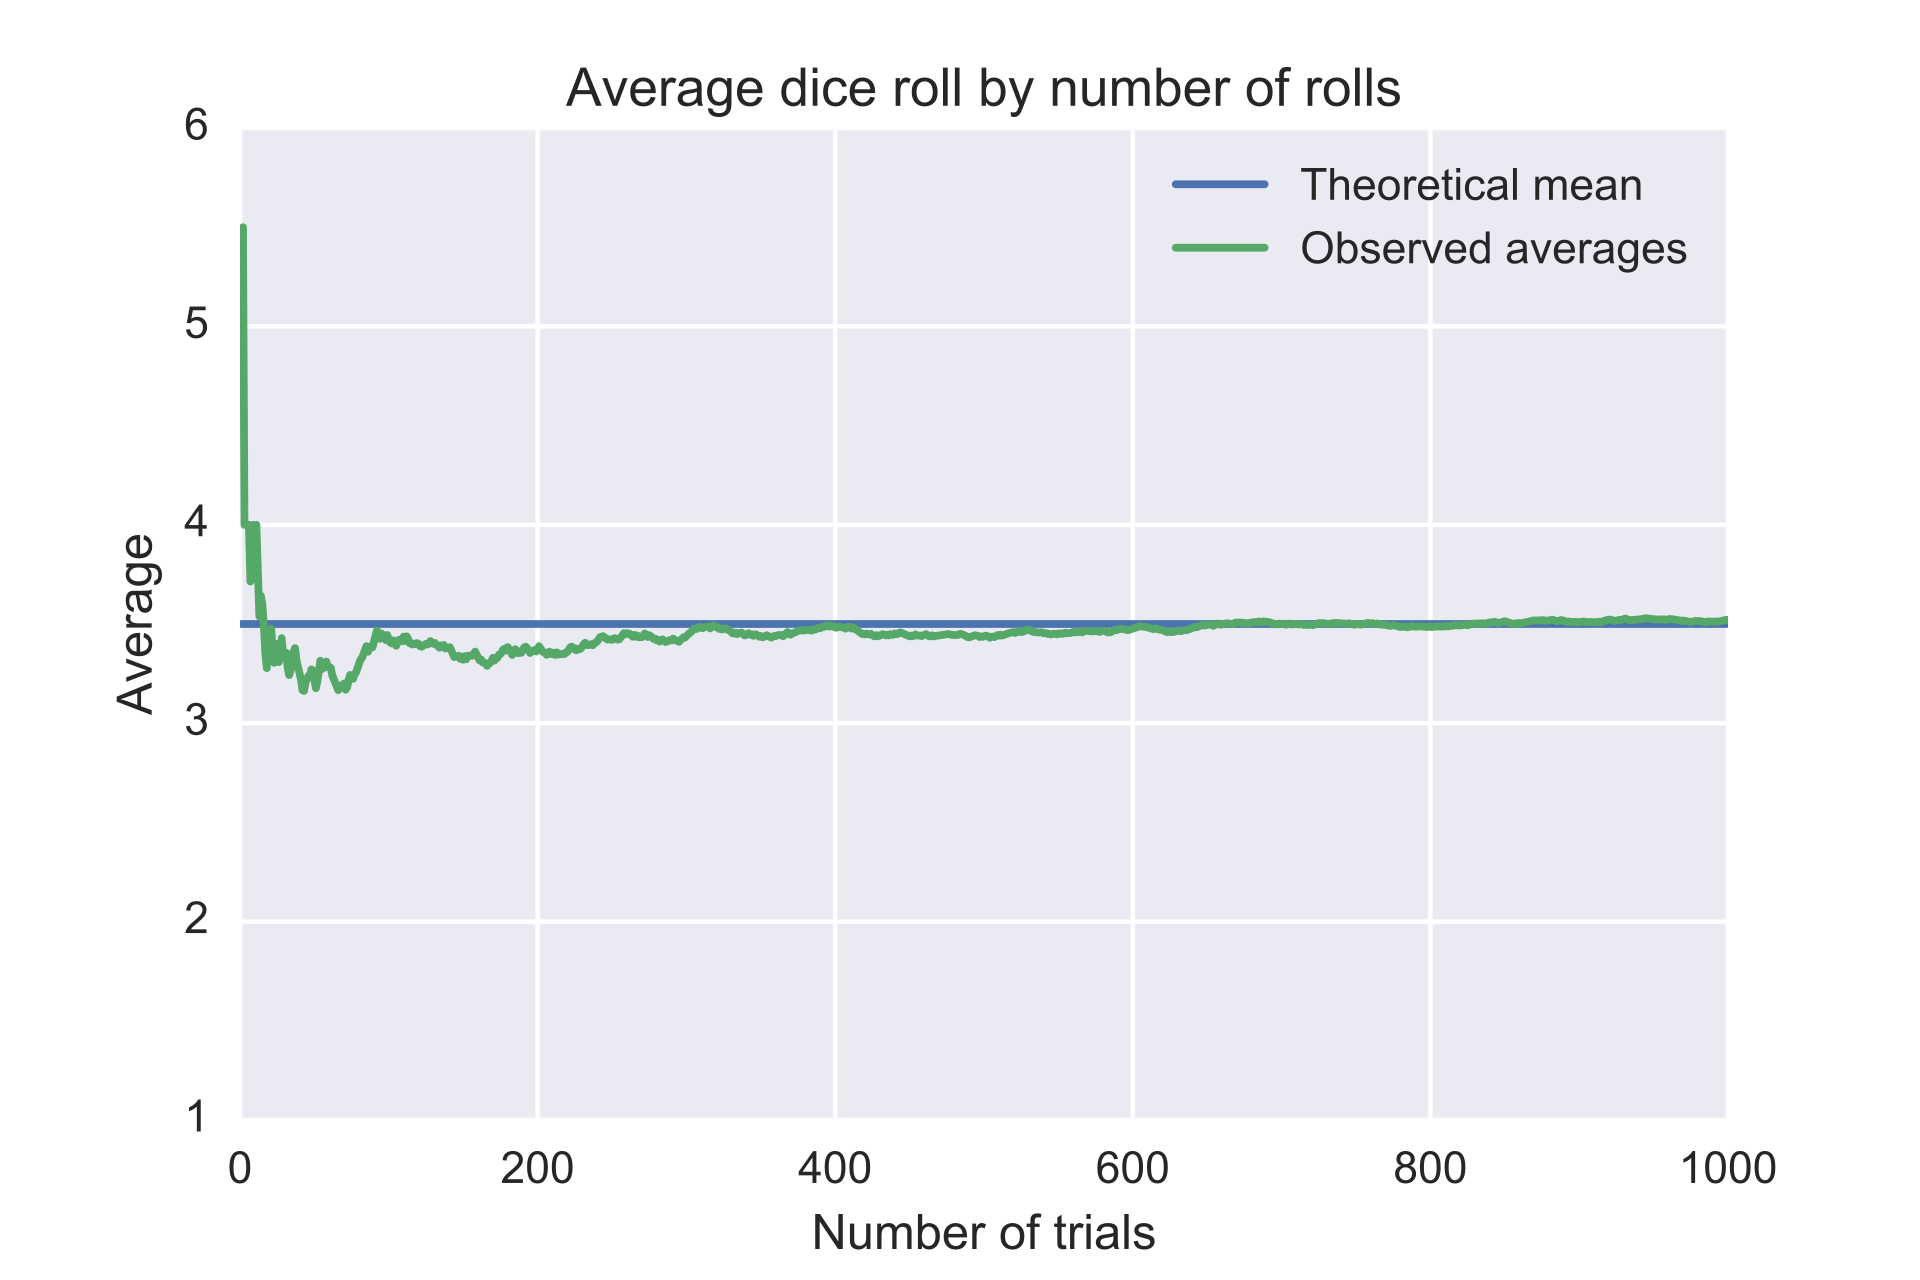
\includegraphics[width=.8\textwidth]{figures/figure1.png}
    \caption{Illustration de la loi des grands nombres}
\end{figure}

\begin{thm}[Théorème de Glivenko-Contelli, théorème fondamentale de la statistique]
    Soit $ (X_i)_{i \in N} $ une suite de v.a. i.i.d. Soit \begin{align*}
        F_n :& R \to [0,1] \\
            & t \mapsto \frac{1}{n}\sum_{i=1}^{n}\mathbbm{1}_{X_i \leq t}
    \end{align*}
    Alors :
    \[
        P(\left\| F_n - F_{X_1} \right\|_{\infty } \to _{n \to \infty } 0 ) = 1
    .\]
    Reformulons: Presque-sûrement, la suite de fonction $ (F_n)_{n \in N} $ converge uniformément vers $ F_{X_1} $.
\end{thm}

\textbf{Rappel : } $ F_n \to ^{CV}_{n \to + \infty } F $ si $ \left\| F_n -F \right\| _{\infty} \sup \left| F_n(x) - F(x)\right| \to_{n \to + \infty } 0$  Si on aime les quantificateurs : 
\[
    \forall \epsilon > 0, \exists N \in \mathbb{N}, \forall t \in R, \left| F_n(t) - F(t) \right| < \epsilon 
.\]

\begin{figure}[htbp]
    \centering
    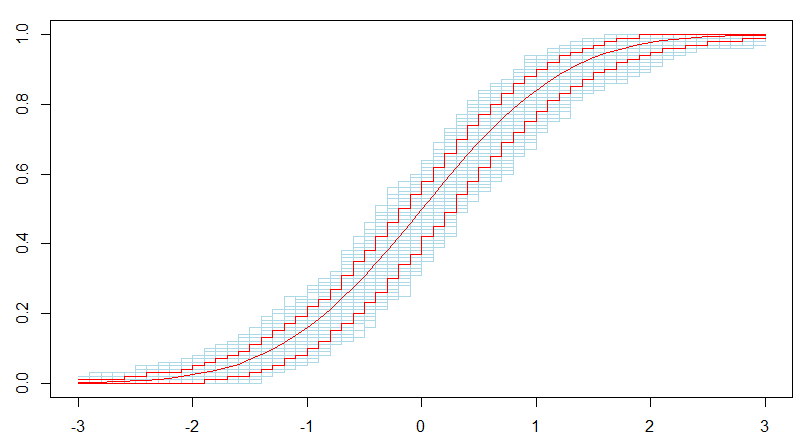
\includegraphics[width=\textwidth]{figures/figure2.png}
    \caption{Illustration du théorème de Glivenko-Contelli}
\end{figure}










\end{document}